\documentclass[professionalfonts]{beamer}
\usepackage[familydefault,light]{Chivo} 
\usepackage[T1]{fontenc}
\usenavigationsymbolstemplate{}
\usepackage[]{hyperref}
\usepackage{tikz,pgf,pgfarrows,pgfnodes,pgfbaseimage}
\graphicspath{{./Pics/}}
\usetikzlibrary{shapes}
\usepackage{setspace}
\newcommand{\evi}[1]{{\colorbox{yellow!50}{{#1}}}}
\newcommand{\exe}[1]{{\color{black!50}{{#1}}}}
\newcommand{\kw}[1]{{\colorbox{black!30}{\color{white}{#1}}}}
\tikzstyle{nd}=[circle,draw=black,thick,minimum size=.8cm,inner sep=1pt]
\setbeamercovered{transparent}
\usetheme{Singapore}
\tikzstyle{nodo}=[ellipse,draw=black!60,fill=black!10,line width=.7pt,minimum width=.7cm,minimum height=.4cm]
\usecolortheme[named=gray]{structure}
\setbeamercolor{block title}{bg=black!20,fg=black}
\setbeamercolor{block body}{bg=black!10,fg=black}

\title{Algoritmi Numerici (Parte I)}
\subtitle{[Lezione 1] Algoritmo di Horner e suo Inverso}
\author{Alessandro Antonucci\\{\tt alessandro.antonucci@supsi.ch}}
\date{\tiny\url{https://colab.research.google.com/drive/1rjCcQMtkfmHeLEm593Ew3JlXm2dEoQSd}}
%%%%%%%%%%%%%%%%%%%%%%%%%%%%
\begin{document}
\maketitle
\frame{\frametitle{Algoritmi}
\setstretch{1.4}
\begin{itemize}
\item Somma dei primi $100$ numeri? $5050$! 
\item Approccio lento $1+2+3+\ldots+98+99+100$ 
\item Approccio veloce $(1+100)+(2+99)+\ldots=101 \times 50$
\end{itemize}
\vskip 1mm
\begin{center}
{\it Dato $n$ (input) calcolare somma $s$ (output) primi $n$ numeri?}
\end{center}
\vskip -2mm
\begin{itemize}
\item Algoritmo ``lento'' esegue $n-1$ addizioni
\\(complessit\`a $O(n)$, ovvero lineare)
\item Algoritmo veloce $s=\frac{n(n+1)}{2}$ (1 somma, 1 molt , 1 div)
\\(complessit\`a $O(1)$, ovvero costante)
\end{itemize}}

\frame{\frametitle{Linguaggi}
\setstretch{1.4}
\begin{itemize} 
\item Linguaggio = sistema codificato di simboli che permette di esprimere un insieme di concetti
\item Linguaggio numerico = sistema codificato di simboli che permette di esprimere gli elementi di un insieme numerico
\end{itemize}
Es. rappresentazione numeri (naturali) in base 10\\
\begin{center}
{\it \small  Simboli = $\{0,1,2,3,4,5,6,7,8,9\}$ , Codice = sistema posizionale}
\\[2mm]
$4273 = 4\times 1000 + 2\times 100 + 7\times 10 + 3$
\\[1mm]
$4273 = 4\times 10^3 + 2\times 10^2 + 7\times 10^1 + 3 \times 10^0$
\end{center}}

\frame{\frametitle{Un algoritmo di lettura per i numeri in base 10}
\setstretch{1.1}
\begin{itemize} 
\item Numero rappresentato come array (vettore) di digits (cifre)\\
{\centering $k=(d_n,d_{n-1},\ldots,d_1,d_0)$}
\item Formula di lettura $k=\sum_{i=0}^n d_i \times 10^i$
\item Dalla formula al(lo pseudo) codice
\end{itemize}
\centering
\begin{tabular}{p{8cm}}
{\tt output = 0}\\
{\tt input = d(n),d(n-1), $\ldots$ d(1),d(0)}\\
{\tt for  = 0 $\ldots$ n}\\
{\tt \quad \quad output = output + d(i) * 10**i}\\
{\tt end}\\
{\tt return output}
\end{tabular}}

\frame{\frametitle{L'algoritmo di Horner (base 10)}
\setstretch{1.1}
\begin{itemize} 
\item $4273 = ((4\times10+2)\times 10 +7)\times10+3$
\item Schema di lettura pi\`u rapido
\end{itemize}
\centering
\begin{tabular}{p{8cm}}
{\tt input = d(n),d(n-1), $\ldots$ d(1),d(0)}\\
{\tt output = d(n)}\\
{\tt for i = n-1 $\ldots$ 0}\\
{\tt \quad \quad output = output * 10 +  d(i)}\\
{\tt end}\\
{\tt return output}
\end{tabular}
\vskip 2mm
\begin{itemize}
\item Complessit\`a $O(n)$ (lineare) anzich\'e quadratica!
\item Funziona in qualunque base!
\end{itemize}}

\frame{\frametitle{L'algoritmo di Horner (base b)}
\setstretch{1.1}
\begin{itemize} 
\item $1302_4 = 1\times 4^3 + 3\times 4^2 + 0 \times 4^1 + 2 \times 4^0 = 114_{10}$
\item $1302_4=((1\times 4+3)\times 4 + 0)\times 4 + 2 = 114_{10}$
\item $(d_n,d_{n-1},\ldots,d_1,d_0)=\sum_{i=0}^n d_i \times b^i$
\end{itemize}
\centering
\begin{tabular}{p{8cm}}
{\tt input = d(n),d(n-1), $\ldots$ d(1),d(0)}\\
{\tt output = d(n)}\\
{\tt for i = n-1 $\ldots$ 0}\\
{\tt \quad \quad output = output * b +  d(i)}\\
{\tt end}\\
{\tt return output}
\end{tabular}
\begin{itemize}
\item L'algoritmo converte in base $10$ un numero in base $b$
\end{itemize}}

\frame{\frametitle{L'operatore modulo}
\setstretch{1.4}
\begin{itemize}
\item $n \mod m$ \`e il resto della divisione intera di $n$ per $m$
\item sottraggo $m$ a $n$ finch\'e non ottengo un numero $<m$,
\item $n \mod m$ \`e un numero compreso fra $0$ e $m-1$
\item Es. $n \mod 2$ \`e $0$ per $n$ pari ed $1$ per $n$ dispari
\item Es. $n \mod 3$ \`e $0$ per $n$ multiplo di $3$, $1$ se $n-1$ \`e multiplo di $3$, $2$ se $n+1$ \`e multiplo di $3$
\item Es. $n \mod 10$ \`e la cifra pi\`u a destra di $n$
\end{itemize}

}
\frame{\frametitle{L'inverso dell'algoritmo di Horner}
\setstretch{1.1}
\begin{itemize}
\item Convertire in base $b$ un numero in base $10$?
\item Invertire l'algoritmo di Horner!
\item $114_{10} = \ldots_4$?
\vskip 3mm
\begin{tabular}{p{3cm}p{3cm}}
$114 \mod 4 = 2$ &$(114-2)/4=28$\\
$28 \mod 4 = 0$ &$(28-0)/4=7$\\
$7 \mod 4 = 3$ &$(7-3)/4=1$\\
$1 \mod 4 = 1$ &$(1-1)/4=0$\\
\end{tabular}
\item $114_{10} = 1302_4$!
\end{itemize}}





\frame{\frametitle{Da base m a base 10}
\begin{columns}
\begin{column}[T]{0.5\textwidth}
\Large\centering
$100110111_2 = 311_{10}$
\vskip 2mm
$200102_3 = 497_{10}$
\vskip 2mm
$2177_8 = 1151_{10}$
\end{column}
\begin{column}[T]{0.5\textwidth}
\Large\centering
$AC12_{16} = 44050_{10}$
\vskip 2mm
$1111_3 = 40_{10}$
\vskip 2mm
$1111_4 = 85_{10}$
\end{column}
\end{columns}
\vskip 10mm
\centering
Nota: un numero in base $b$ usa le cifre $\{ 0 , 1 , 2 , \ldots , b-1 \}$
\vskip 2mm
Se $b>10$ servono nuove cifre (es. le lettere). \\ Esadecimale $b=16$:
\vskip 2mm
\begin{center}
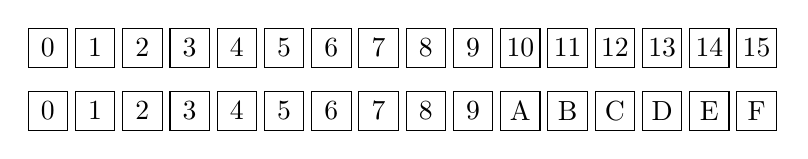
\begin{tikzpicture}
	\foreach \x in {0,1,2,3,4,5,6,7,8,9,10,11,12,13,14,15}
	\draw (\x*0.6,0) +(-.25,-.25) rectangle ++(.25,.25);
	\foreach \x in {0,1,2,3,4,5,6,7,8,9,10,11,12,13,14,15}
	\draw (\x*0.6,0) node{\x};
	\foreach \x in {0,1,2,3,4,5,6,7,8,9,10,11,12,13,14,15}
	\draw (\x*0.6,-.8) +(-.25,-.25) rectangle ++(.25,.25);
	%\foreach \x in {0,1,2,3,4,5,6,7,8,9,10,11,12,13,14,15}
	\foreach \x in {0,1,2,3,4,5,6,7,8,9}
	\draw (\x*0.6,-.8) node{\x};
	\draw (10*0.6,-.8) node{A};
	\draw (11*0.6,-.8) node{B};
	\draw (12*0.6,-.8) node{C};
	\draw (13*0.6,-.8) node{D};
	\draw (14*0.6,-.8) node{E};
	\draw (15*0.6,-.8) node{F};
\end{tikzpicture}
\end{center}}

\frame{\frametitle{Da base 10 a base n}
\begin{columns}
\begin{column}[T]{0.5\textwidth}
\Large\centering
$2143_{10} =100001011111_{2}$
\vskip 2mm
$13458_{10} = 3492_{16}$
\vskip 2mm
$798_{10} = 1436_{8}$
\end{column}
\begin{column}[T]{0.5\textwidth}
\Large\centering
$144_{10} = 10010000_{2}$
\vskip 2mm
$144_{10} = 12100_{3}$
\vskip 2mm
$144_{10} = 2100_{4}$
\end{column}
\end{columns}
}
\frame{\frametitle{Da base m a base n}
\begin{center}
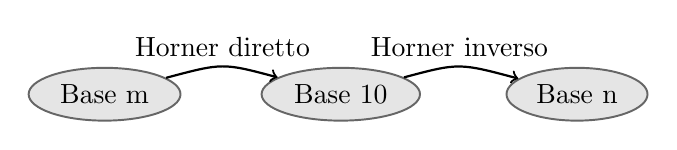
\begin{tikzpicture}
\node[nodo] (a)  at (0,0) {Base m};
\node[nodo] (b)  at (3,0) {Base 10};
\node[nodo] (c)  at (6,0) {Base n};
\draw[->,above,thick] (a) .. controls (1.5,.4) ..  (b) node[midway] {Horner diretto};
\draw[->,above,thick] (b) .. controls (4.5,.4) ..  (c) node[midway] {Horner inverso};
%\draw[->,below,thick] (d) .. controls (2.5,-.4) .. (b) node[midway] {Inverso};
\end{tikzpicture}
\end{center}
\begin{itemize}\Large
	\item $1032_4 = 78_{10} = 2220_{3}$
	\item $101101_2 = 45_{10} = 140_{5}$
	\item $2177_8 = 1151_{10} = 47F_{16}$
\end{itemize}
}
\frame{\frametitle{Da base m a base n (trasformazioni dirette)}
\Large
$210745_{10}=\ldots_{100}?$
\vskip 2mm
$2 \cdot 10^5 +1 \cdot 10^4 +0 \cdot 10^3 + 7 \cdot 10^2 + 4 \cdot 10^1 + 5 \cdot 10^0=$
\vskip 2mm
$21 \cdot 100^2 + 7 \cdot 100^1 + 45 \cdot 100^0 $
\vskip 2mm
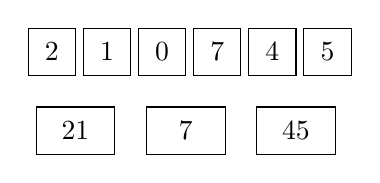
\begin{tikzpicture}
	\draw (0,0) +(-.3,-.3) rectangle ++(.3,.3);
	\draw (.7,0) +(-.3,-.3) rectangle ++(.3,.3);
	\draw (1.4,0) +(-.3,-.3) rectangle ++(.3,.3);
	\draw (2.1,0) +(-.3,-.3) rectangle ++(.3,.3);
	\draw (2.8,0) +(-.3,-.3) rectangle ++(.3,.3);
	\draw (3.5,0) +(-.3,-.3) rectangle ++(.3,.3);
	\draw (.3,-1) +(-.5,-.3) rectangle ++(.5,.3);
	\draw (1.7,-1) +(-.5,-.3) rectangle ++(.5,.3);
	\draw (3.1,-1) +(-.5,-.3) rectangle ++(.5,.3);
	\draw (0,0) node{2};
	\draw (.7,0) node{1};
	\draw (1.4,0) node{0};
	\draw (2.1,0) node{7};
	\draw (2.8,0) node{4};
	\draw (3.5,0) node{5};
	\draw (.3,-1) node{21};
	\draw (1.7,-1) node{7};
	\draw (3.1,-1) node{45};
\end{tikzpicture}
\vskip 2mm
$100 = 10^2$: cifre raggruppate a due a due
\vskip 3mm
Stessa cosa se base $b$ e non $10$
}
\frame{\frametitle{Da binario ad hexa (e viceversa)}
\begin{itemize}\Large
	\item $1032_4 = 1001110_{2}$
	\item $101101_2 = 2D_{16}$
	\item $2177_8 = 010001111111_{2}$
\end{itemize}}

\frame{\frametitle{Esercitazione (Esercizio 1)}
\setstretch{1.4}
Eseguire i seguenti cambiamenti di base
\Large
\begin{itemize}
\item $2177_8=\ldots_2${\small$\color{black!20}{(=1151_{10}=10001111111_2})$}
\item $10220_3=\ldots_9${\small$\color{black!20}{(=105_{10}=126_9})$}
\item $20016_7=\ldots_5${\small$\color{black!20}{(=4815_{10}=123230_5})$}
\item $AC12_{16}=\ldots_8${\small$\color{black!20}{(=44050_{10}=126022_8})$}

\end{itemize}}

\frame{\frametitle{Esercitazione (Esercizio 2)}
\setstretch{1.4}
Eseguire i seguenti cambiamenti di base
\begin{itemize}
\item $1111_2=\color{black!20}{15_{10}}$, $11111_2=\color{black!20}{31_{10}}$, $111111_2=\color{black!20}{63_{10}}$ 
\item $222_3=\color{black!20}{26_{10}}$, $2222_3=\color{black!20}{80_{10}}$, $22222_3=\color{black!20}{242_{10}}$, 
\item $44_5=\color{black!20}{24_{10}}$, $444_5=\color{black!20}{124_{10}}$, $4444_5=\color{black!20}{624_{10}}$, 
\vskip 3mm
\begin{center}
${\underbrace{bbbb \ldots bb_{b+1}}_{\text{n cifre}}}=(b+1)^n-1$%{b+1}$%% = \ldots_{10}$
\end{center}
\end{itemize}}

\frame{\frametitle{Esercitazione (Esercizio 3)}
\setstretch{1.2}
\normalsize
In C una variabile {\tt unsigned int} richiede al compilatore di allocare 32 bit, che verranno utilizzati per rappresentare numeri interi senza segno secondo le regole del sistema posizionale in base due
\vskip 1mm
{\tt unsigned short/long} fanno lo stesso con 16/64 bit. 
\small
\begin{itemize}
\item Rappresentare il numero 131'086 nei tre formati
\item Identificare il pi\`u grande numero in ogni formato
\item Leggere le sequenze (compattate)
\begin{center}
$A019$ $\color{black!20}{(=40985_{10}})$ {\tt unsigned short}\\
$010C|7142$ $\color{black!20}{(=17592642_{10})}$ {\tt unsigned int}\\
$0000|100A|0007|3501$ $\color{black!20}{(\simeq 1.765 \cdot 10^{13})}$ {\tt unsigned long}\\
\end{center}
\end{itemize}}
\end{document}
